\section{环空间与割空间}
\label{sec:graph-cycle-cut-spaces}

上一节建立了关联矩阵的两种对偶运算：沿边差分算子$\bm{B}^\top\colon\mathbb{R}^V\to\mathbb{R}^E$把顶点函数变成沿边差分向量，净流出汇总算子$\bm{B}\colon\mathbb{R}^E\to\mathbb{R}^V$把边流量向量变成各顶点的净流出量。这两个算子在边空间$\mathbb{R}^E$中自然划分出两类核心子空间——在所有顶点处净流出均为零的边流量构成环空间$\ker\bm{B}$，由顶点函数沿边差分生成的边向量构成割空间$\operatorname{im}\bm{B}^\top$。

本节依次建立这两个子空间的定义、正交直和分解与维数公式，最后利用生成森林构造出两组可直接读出坐标的显式基。

\subsection{环空间}
\label{sec:incidence-cycle-space}

我们先在图~\ref{fig:incidence-running-example}的四点五边图上考察什么样的边流量向量能使每个顶点的净流出量都等于零。

第一股流量沿外圈四元环$1\to2\to3\to4\to1$依次输送$1$个单位，对角边$13$上不送流。在每个顶点处核对进出账目：在顶点$1$，边$12$流出$1$个单位、边$41$流入$1$个单位，净流出为零；在顶点$2$，边$12$流入$1$个单位、边$23$流出$1$个单位，净流出也为零；顶点$3$与顶点$4$同理。因为外圈四条边的绕行方向与图~\ref{fig:incidence-running-example}约定的参考方向完全一致，按边序$(12,23,34,41,13)$记录，这股边流量向量为
\[
\bm{c}_1=(1,1,1,1,0)^\top.
\]
代入关联矩阵直接验算，确实有$\bm{B}\bm{c}_1=\bm{0}$。

第二股流量沿三角形回路$1\to3\to2\to1$绕行$1$个单位，外圈边$34$和$41$上不送流。逐边核对绕行方向与参考方向的关系：在对角边$13$上，绕行从$1$到$3$，与参考方向$1\to3$一致，分量取$+1$；在边$23$和边$12$上，绕行分别从$3$到$2$、从$2$到$1$，均与各自的参考方向（$2\to3$和$1\to2$）相反，分量均取$-1$；边$34$与$41$不在该三角形回路上，分量均取$0$。于是这股三角形环流写成边流量向量为
\[
\bm{c}_2=(-1,-1,0,0,1)^\top.
\]
逐行计算$\bm{B}\bm{c}_2$，每个顶点的流入与流出同样精确抵消，满足$\bm{B}\bm{c}_2=\bm{0}$。

由于矩阵乘法是线性的，两股处处守恒的边流量相加后依然满足守恒条件：$\bm{B}(\bm{c}_1+\bm{c}_2)=\bm{B}\bm{c}_1+\bm{B}\bm{c}_2=\bm{0}$。把两个向量逐分量相加：
\[
\bm{c}_1+\bm{c}_2=(1,1,1,1,0)^\top+(-1,-1,0,0,1)^\top=(0,0,1,1,1)^\top.
\]
图~\ref{fig:incidence-circulation-superposition}展示了这一叠加过程：在公共边$12$和$23$上，$\bm{c}_1$的正向单位流$+1$与$\bm{c}_2$的反向单位流$-1$恰好正反抵消、合成为零流量；剩下的三条边$34,41,13$首尾相接，恰好构成沿右下方三角形$1\to3\to4\to1$绕行的单位环流。同理，将任意守恒流量乘以实数倍，在每个顶点处的流入和流出按同一比例缩放，净流出量仍然为零。

\begin{BookInlineFigure}
  \centering
  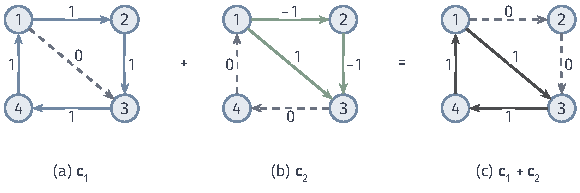
\includegraphics{figures/03-graphs/05-matrices-and-spectra/tikz/incidence-circulation-superposition/figure.pdf}
  \caption{四点五边图上两股环流的叠加$\bm{c}_1+\bm{c}_2$。边旁数字为对应参考方向下的流量分量，虚线表示流量为零。(a) 沿外圈$1\to2\to3\to4\to1$的单位环流$\bm{c}_1$。(b) 沿三角形$1\to3\to2\to1$的单位环流$\bm{c}_2$，其中边$12,23$因逆参考方向而取$-1$。(c) 叠加结果在边$12,23$上正反抵消为零，化为沿三角形$1\to3\to4\to1$的单位环流。}
  \label{fig:incidence-circulation-superposition}
\end{BookInlineFigure}

把“每个顶点处净流出量均为零”这一守恒条件写成一般形式，就得到环流与环空间的严格定义。

\begin{definition}[环流与环空间]
\label{def:graph-cycle-space}
设$\mathcal{G}=(V,E)$为有限图，$\bm{B}\in\mathbb{R}^{n\times m}$为其关联矩阵。若边流量向量$\bm{q}\in\mathbb{R}^E$在每个顶点处的净流出量均为零，即满足
\[
(\bm{B}\bm{q})_v=0\quad(\forall\,v\in V),
\qquad\text{或等价地}\qquad \bm{B}\bm{q}=\bm{0},
\]
则称$\bm{q}$为图$\mathcal{G}$上的一个\term{环流}（circulation）。全体实数环流构成的边空间线性子空间（即关联矩阵$\bm{B}\colon\mathbb{R}^E\to\mathbb{R}^V$的零空间）称为图$\mathcal{G}$的\term{环空间}（cycle space），记为
\begin{equation}
\mathcal{C}(\mathcal{G})=\{\bm{q}\in\mathbb{R}^E:\bm{B}\bm{q}=\bm{0}\}
=\ker\bm{B}.
\label{eq:incidence-cycle-space}
\end{equation}
\end{definition}

需要注意，本章定义的环空间$\mathcal{C}(\mathcal{G})$是实数域$\mathbb{R}$上的线性子空间：每条边可以承载任意实数大小的流量，负分量表示流向与参考方向相反。这与组合图论中在二元域$\mathbb{F}_2$（模$2$加法）下讨论的边子集对称差不同——在实数环空间中，两股同向的单位环流相加会变成$2$倍流量的环流，只有方向相反、大小相等的两股流量叠加才会抵消为零。

一般而言，环空间$\mathcal{C}(\mathcal{G})$中的元素既可以是沿单个简单环绕行的流量，也可以是由多个不同环路按任意实系数线性叠加而成的复合守恒流。那么，任意一个复杂的环流是否都能由少数几个基本简单环线性表出？第~\ref{sec:incidence-fundamental-bases}小节将利用生成森林给出肯定的回答与具体构造方法。在此之前，我们先考察边空间中由沿边差分生成的另一半子空间。

\subsection{割空间}
\label{sec:incidence-cut-space}

现在从相反的方向在边空间$\mathbb{R}^E$中生成向量：先给定顶点函数$\bm{f}\in\mathbb{R}^V$，再通过沿边差分算子$\bm{B}^\top$计算沿边差分向量$\bm{d}=\bm{B}^\top\bm{f}\in\mathbb{R}^E$。

最简单的一类顶点函数是将顶点集$V$分成两部分、在一侧赋$1$而在另一侧赋$0$的指示函数。任取顶点子集$S\subseteq V$，记其补集为$\bar{S}=V\setminus S$，令指示向量$\bm{1}_S\in\mathbb{R}^V$在$S$内的顶点上取$1$、在$\bar{S}$内的顶点上取$0$。对$\bm{1}_S$作用沿边差分算子，得到边空间中的列向量
\[
\bm{d}_S=\bm{B}^\top\bm{1}_S\in\mathbb{R}^E.
\]
对任意一条参考方向为$e\colon u\to v$的边，其分量$(\bm{d}_S)_e=\bm{1}_S(u)-\bm{1}_S(v)$只有三种可能取值：
\begin{itemize}
\item 若$u\in S$且$v\in\bar{S}$（边沿参考方向从$S$穿出到$\bar{S}$），则$(\bm{d}_S)_e=1-0=+1$；
\item 若$u\in\bar{S}$且$v\in S$（边沿参考方向从$\bar{S}$穿入到$S$），则$(\bm{d}_S)_e=0-1=-1$；
\item 若$u,v$同属于$S$或同属于$\bar{S}$（边不跨越割$(S,\bar{S})$），则$(\bm{d}_S)_e=0$。
\end{itemize}
因此，$\bm{d}_S$只在跨越割$(S,\bar{S})$的边上非零，称为对应于顶点子集$S$的\emph{割向量}（或带符号割指示向量）。

以四点五边图上的子集$S=\{1,2\}$及其补集$\bar{S}=\{3,4\}$为例。此时顶点指示向量为$\bm{1}_S=(1,1,0,0)^\top$。按边序$(12,23,34,41,13)$逐条检查五条边的端点位置：边$12$（$1\to2$）两端都在$S$内，差值为$1-1=0$；边$34$（$3\to4$）两端都在$\bar{S}$内，差值为$0-0=0$；边$23$（$2\to3$）和边$13$（$1\to3$）分别从$S$内的顶点$2,1$指向$\bar{S}$内的顶点$3$，差值均为$1-0=+1$；边$41$（$4\to1$）从$\bar{S}$内的$4$指向$S$内的$1$，差值为$0-1=-1$。汇总起来，子集$S=\{1,2\}$生成的割向量为
\[
\bm{d}_S=\bm{B}^\top\bm{1}_S=(0,1,0,-1,1)^\top\in\mathbb{R}^5.
\]
图~\ref{fig:incidence-cut-vector-example}直观展示了这一过程：左图以虚线将顶点集划分为上侧$S=\{1,2\}$（读数$1$）与下侧$\bar{S}=\{3,4\}$（读数$0$）；右图标出经$\bm{B}^\top$作用后各边上的差分分量，内部边$12,34$分量为$0$，三条跨割边$23,41,13$按穿行方向分别取$+1,-1,+1$。

\begin{BookInlineFigure}
  \centering
  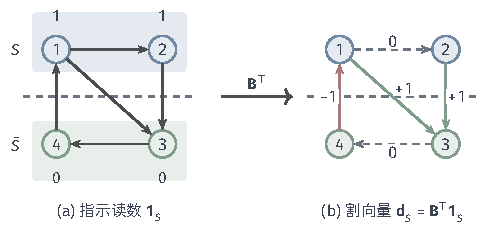
\includegraphics{figures/03-graphs/05-matrices-and-spectra/tikz/incidence-cut-vector-example/figure.pdf}
  \caption{四点五边图上子集$S=\{1,2\}$对应的割向量构造。(a) 将顶点划分为$S=\{1,2\}$（蓝底，赋读数$1$）与$\bar{S}=\{3,4\}$（绿底，赋读数$0$），构成顶点指示向量$\bm{1}_S=(1,1,0,0)^\top$。(b) 经沿边差分算子$\bm{B}^\top$作用后得到的割向量$\bm{d}_S=(0,1,0,-1,1)^\top$：同侧边$12,34$（虚线）差值为$0$，从$S$指向$\bar{S}$的跨割边$23,13$（绿线）取$+1$，从$\bar{S}$指向$S$的跨割边$41$（红线）取$-1$。}
  \label{fig:incidence-cut-vector-example}
\end{BookInlineFigure}

不仅$0$--$1$指示函数如此，任意一个实值顶点函数$\bm{f}\in\mathbb{R}^V$都可以按单点指示向量（即标准基向量$\bm{1}_{\{v\}}=\bm{e}_v$）展开为$\bm{f}=\sum_{v\in V}f(v)\bm{1}_{\{v\}}$。利用矩阵乘法的线性性，它的沿边差分向量可以写成
\[
\bm{B}^\top\bm{f}
=\sum_{v\in V}f(v)\,\bm{B}^\top\bm{1}_{\{v\}}
=\sum_{v\in V}f(v)\,\bm{d}_{\{v\}}.
\]
上式右端每一项都是单点割向量$\bm{d}_{\{v\}}=\bm{B}^\top\bm{1}_{\{v\}}$的数乘。这说明：任意顶点函数的沿边差分向量都是割向量的线性组合；反过来，任意一组割向量的线性组合$\sum_k\alpha_k\bm{B}^\top\bm{1}_{S_k}=\bm{B}^\top\bigl(\sum_k\alpha_k\bm{1}_{S_k}\bigr)$也必定是某个顶点函数的沿边差分向量。由此我们给出割空间的形式化定义。

\begin{definition}[割空间]
\label{def:graph-cut-space}
设$\mathcal{G}=(V,E)$为有限图，$\bm{B}\in\mathbb{R}^{n\times m}$为其关联矩阵。若边向量$\bm{d}\in\mathbb{R}^E$可以表示为某个顶点函数$\bm{f}\in\mathbb{R}^V$的沿边差分向量，即存在$\bm{f}\in\mathbb{R}^V$使得
\[
\bm{d}=\bm{B}^\top\bm{f}\qquad\bigl(\text{即对每条边 }e\colon u\to v\text{ 有 }d_e=f(u)-f(v)\bigr),
\]
则称$\bm{d}$为图$\mathcal{G}$上的一个沿边差分向量（或割差分向量）。全体顶点函数的沿边差分向量构成的边空间线性子空间（即沿边差分算子$\bm{B}^\top\colon\mathbb{R}^V\to\mathbb{R}^E$的像空间）称为图$\mathcal{G}$的\term{割空间}（cut space），记为
\begin{equation}
\mathcal{D}(\mathcal{G})=\{\bm{B}^\top\bm{f}:\bm{f}\in\mathbb{R}^V\}=\operatorname{im}\bm{B}^\top.
\label{eq:incidence-cut-space}
\end{equation}
\end{definition}

\paragraph{正交直和分解}

把定义~\ref{def:graph-cycle-space}与定义~\ref{def:graph-cut-space}放在一起，一个核心几何事实立刻浮现：环空间$\mathcal{C}(\mathcal{G})=\ker\bm{B}$与割空间$\mathcal{D}(\mathcal{G})=\operatorname{im}\bm{B}^\top$在边空间$\mathbb{R}^E$中正交互补。

先验证正交性。任取一个环流$\bm{c}\in\mathcal{C}(\mathcal{G})=\ker\bm{B}$和一个沿边差分向量$\bm{d}=\bm{B}^\top\bm{f}\in\mathcal{D}(\mathcal{G})$。根据式~\eqref{eq:incidence-adjoint-pairing}的伴随恒等式，二者在边空间中的内积为
\[
\langle\bm{d},\bm{c}\rangle_E
=\langle\bm{B}^\top\bm{f},\bm{c}\rangle_E
=\langle\bm{f},\bm{B}\bm{c}\rangle_V
=\langle\bm{f},\bm{0}\rangle_V=0,
\]
其中倒数第二步直接使用了环流的守恒条件$\bm{B}\bm{c}=\bm{0}$。

用简单环路可以直观看出两个向量内积为何恒为零。比如沿三角形$1\to2\to3\to1$绕行一圈的单位环流，将它与任意顶点函数$\bm{f}$的沿边差分作内积，相当于把沿环三步的端点差逐段相加：
\[
\bigl(f(1)-f(2)\bigr)+\bigl(f(2)-f(3)\bigr)+\bigl(f(3)-f(1)\bigr)=0.
\]
环上的每个顶点读数恰好出现两次——在离开该点的一步中取正号，在进入该点的一步中取负号——绕行闭合回路一圈后必然首尾相消（对应物理学中的基尔霍夫电压定律：保守势场沿任意闭合回路的电势降之和为零）。

不仅如此，割空间$\mathcal{D}(\mathcal{G})$的正交补$\mathcal{D}(\mathcal{G})^\perp$恰好就是整个环空间$\mathcal{C}(\mathcal{G})$。事实上，设边向量$\bm{q}\in\mathbb{R}^E$与割空间中的每一个沿边差分向量都正交，即对任意$\bm{f}\in\mathbb{R}^V$都有
\[
0=\langle\bm{B}^\top\bm{f},\bm{q}\rangle_E=\langle\bm{f},\bm{B}\bm{q}\rangle_V.
\]
由于上式对所有顶点函数$\bm{f}\in\mathbb{R}^V$均成立，特别地取$\bm{f}=\bm{B}\bm{q}\in\mathbb{R}^V$，即得
\[
\lVert\bm{B}\bm{q}\rVert_2^2=\langle\bm{B}\bm{q},\bm{B}\bm{q}\rangle_V=0,
\]
从而$\bm{B}\bm{q}=\bm{0}$，说明$\bm{q}\in\ker\bm{B}=\mathcal{C}(\mathcal{G})$。在有限维欧氏空间中，任意子空间与其正交补构成整个空间的正交直和（可参考\BookChapterRef{chap:inner-product-spaces}{卷二"内积空间"章}），因此边空间$\mathbb{R}^E$具有正交直和分解：
\begin{equation}
\mathbb{R}^E=\mathcal{C}(\mathcal{G})\oplus\mathcal{D}(\mathcal{G})
=\ker\bm{B}\oplus\operatorname{im}\bm{B}^\top.
\label{eq:incidence-edge-space-decomposition}
\end{equation}

式~\eqref{eq:incidence-edge-space-decomposition}表明，图上的任意边向量$\bm{q}\in\mathbb{R}^E$都可以唯一地分解为一个守恒环流$\bm{c}\in\mathcal{C}(\mathcal{G})$与一个沿边差分向量$\bm{d}\in\mathcal{D}(\mathcal{G})$之和：$\bm{q}=\bm{c}+\bm{d}$且$\langle\bm{c},\bm{d}\rangle_E=0$。分解的唯一性由正交性直接保证：若另有$\bm{q}=\bm{c}'+\bm{d}'$，相减得$\bm{c}-\bm{c}'=\bm{d}'-\bm{d}$；该差向量同时属于相互正交的$\mathcal{C}(\mathcal{G})$与$\mathcal{D}(\mathcal{G})$，故与自身的内积为零，只能是零向量。

我们用四点五边图上的边向量$\bm{q}=(1,2,1,0,1)^\top$验证这一正交分解：
\[
\bm{q}=\underbrace{(1,1,1,1,0)^\top}_{\bm{c}_1\in\mathcal{C}(\mathcal{G})}
      +\underbrace{(0,1,0,-1,1)^\top}_{\bm{d}_S\in\mathcal{D}(\mathcal{G})},
\]
其中第一项是外圈单位环流$\bm{c}_1$，第二项是子集$S=\{1,2\}$生成的割向量$\bm{d}_S$。容易核对$\langle\bm{c}_1,\bm{d}_S\rangle_E=0+1+0-1+0=0$。例如在边$41$上，环流分量$+1$与割差分分量$-1$叠加后恰好给出$q_{41}=0$；在边$23$上，两项同为$+1$，叠加给出$q_{23}=2$。图~\ref{fig:incidence-flow-decomposition}在三个并排面板中展示了$\bm{q}$、$\bm{c}_1$与$\bm{d}_S$的逐边分量关系。

\begin{BookInlineFigure}
  \centering
  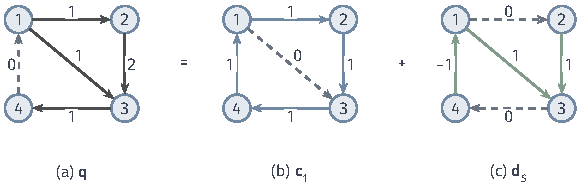
\includegraphics{figures/03-graphs/05-matrices-and-spectra/tikz/incidence-flow-decomposition/figure.pdf}
  \caption{四点五边图上的边向量正交分解$\bm{q}=\bm{c}_1+\bm{d}_S$，其中$S=\{1,2\}$。每条边旁的数值是对应参考方向下的边分量，虚线表示分量为零。}
  \label{fig:incidence-flow-decomposition}
\end{BookInlineFigure}

需要指出的是：虽然边向量$\bm{q}$分解出的沿边差分分量$\bm{d}\in\mathcal{D}(\mathcal{G})$是唯一的，但满足$\bm{B}^\top\bm{f}=\bm{d}$的原像顶点函数$\bm{f}\in\mathbb{R}^V$并不唯一——给$\bm{f}$加上任意属于零空间$\ker\bm{B}^\top$的向量，沿边差分向量$\bm{B}^\top\bm{f}$都保持不变。下一小节通过刻画$\ker\bm{B}^\top$的具体结构，精确算出关联矩阵的秩以及环空间、割空间的维数。

\subsection{子空间维数}
\label{sec:incidence-rank-dimensions}

要计算割空间$\mathcal{D}(\mathcal{G})=\operatorname{im}\bm{B}^\top$与环空间$\mathcal{C}(\mathcal{G})=\ker\bm{B}$各自的维数，关键在于先搞清楚：什么样的顶点函数$\bm{f}\in\mathbb{R}^V$在经过沿边差分算子$\bm{B}^\top$作用后会变成零向量？也就是说，零空间$\ker\bm{B}^\top=\{\bm{f}\in\mathbb{R}^V:\bm{B}^\top\bm{f}=\bm{0}\}$具有什么结构、维数是多少？下面我们分四步把推理过程完整展开。

\paragraph{第一步：同一连通分量内的顶点读数必定相等}

根据沿边差分的定义式~\eqref{eq:incidence-edge-difference}，$\bm{B}^\top\bm{f}=\bm{0}$等价于在每一条边$e\colon u\to v\in E$上都有
\[
f(u)-f(v)=0,\qquad\text{即}\qquad f(u)=f(v).
\]
这表明，只要两个顶点之间有一条边直接相连，它们的读数就必须相等。更进一步，如果两个顶点$i$和$j$属于图的同一个连通分量，那么按连通性的定义，图中存在一条连接$i$与$j$的路径$i=w_0,w_1,\ldots,w_s=j$，其中相邻两步$\{w_{r-1},w_r\}$都是图中的边。沿这条路径逐边应用“相邻端点读数相等”，便得到传递链：
\[
f(i)=f(w_0)=f(w_1)=\cdots=f(w_s)=f(j).
\]
因此，任何满足$\bm{B}^\top\bm{f}=\bm{0}$的顶点函数$\bm{f}$，在图的每一个连通分量内部都必须取同一个常数值。

\paragraph{第二步：不同连通分量之间的常数可以彼此独立选取}

如果整张图$\mathcal{G}$是连通的（只有$1$个连通分量），那么上面第一步已经说明所有$n$个顶点的读数都必须等于同一个常数$\alpha_1$。但如果图$\mathcal{G}$不连通，设它的顶点集$V$划分为$c$个互不相交的连通分量（connected components）：
\[
V=V_1\cup V_2\cup\cdots\cup V_c.
\]
为什么每个连通分量$V_k$可以各自独立地任选一个常数$\alpha_k\in\mathbb{R}$，而不会违反$\bm{B}^\top\bm{f}=\bm{0}$？

原因在于：不同连通分量$V_k$与$V_\ell$（$k\neq\ell$）之间没有任何边相连。换言之，图$\mathcal{G}$中的每一条边$e\colon u\to v\in E$，其两个端点$u$和$v$必定同时落在某一个连通分量$V_k$内部，绝不会出现一端在$V_k$、另一端在$V_\ell$的跨分量边。于是，只要我们在第$1$个连通分量$V_1$的所有顶点上统一赋常数$\alpha_1$，在第$2$个连通分量$V_2$的所有顶点上统一赋常数$\alpha_2$，……，在第$c$个连通分量$V_c$的所有顶点上统一赋常数$\alpha_c$，那么对任意一条边$e\colon u\to v$（不妨设它落在$V_k$内），两端的读数差就恒为
\[
f(u)-f(v)=\alpha_k-\alpha_k=0.
\]
至于其他分量$V_\ell$（$\ell\neq k$）上选了什么常数$\alpha_\ell$，没有边把$\alpha_\ell$和$\alpha_k$连起来作差，因此$\alpha_1,\alpha_2,\ldots,\alpha_c$这$c$个实数彼此之间没有任何耦合约束，可以完全独立地任意取值。特别地，若图中某个顶点$v$是不连任何边的孤立顶点（isolated vertex），它自己单独构成一个连通分量$V_k=\{v\}$；由于没有任何边以$v$为端点，$f(v)=\alpha_k$不出现在$\bm{B}^\top\bm{f}$的任何分量中，也可以独立任取一个实数。

\paragraph{第三步：用分量指示向量表示零空间$\ker\bm{B}^\top$}

为了把“在每个连通分量$V_k$上各自独立取常数$\alpha_k$”写成标准的线性代数语言，我们对第$k$个连通分量$V_k$（$k=1,\ldots,c$）定义其\emph{分量指示向量}$\bm{1}_{V_k}\in\mathbb{R}^V$：
\[
(\bm{1}_{V_k})_v=
\begin{cases}
1,& v\in V_k,\\
0,& v\notin V_k.
\end{cases}
\]
这样，给第$k$个分量的所有顶点赋常数$\alpha_k$，合在一起写成列向量就是线性组合
\begin{equation}
\bm{f}=\alpha_1\bm{1}_{V_1}+\alpha_2\bm{1}_{V_2}+\cdots+\alpha_c\bm{1}_{V_c}.
\label{eq:incidence-ker-bt-expansion}
\end{equation}
我们来逐坐标核对式~\eqref{eq:incidence-ker-bt-expansion}：任取图中的一个顶点$v\in V$，因为$V=V_1\cup\cdots\cup V_c$是互不相交的划分，$v$恰好属于唯一的一个连通分量$V_k$。在顶点$v$所在的坐标位置上，只有$\bm{1}_{V_k}$取$1$，其余$c-1$个指示向量$\bm{1}_{V_\ell}$（$\ell\neq k$）全部取$0$，因此式~\eqref{eq:incidence-ker-bt-expansion}右端在顶点$v$处的值恰好是
\[
\alpha_1\cdot 0+\cdots+\alpha_k\cdot 1+\cdots+\alpha_c\cdot 0=\alpha_k=f(v).
\]
这证明了：$\bm{f}\in\ker\bm{B}^\top$当且仅当$\bm{f}$可以写成式~\eqref{eq:incidence-ker-bt-expansion}的形式。也就是说，这$c$个分量指示向量$\{\bm{1}_{V_1},\ldots,\bm{1}_{V_c}\}$张成了整个零空间$\ker\bm{B}^\top$。

\paragraph{第四步：证明$c$个分量指示向量线性无关}

要确认$\{\bm{1}_{V_1},\ldots,\bm{1}_{V_c}\}$构成$\ker\bm{B}^\top$的一组基，还需证明它们线性无关。设有一组实系数$\alpha_1,\ldots,\alpha_c\in\mathbb{R}$使线性组合等于零向量：
\[
\alpha_1\bm{1}_{V_1}+\alpha_2\bm{1}_{V_2}+\cdots+\alpha_c\bm{1}_{V_c}=\bm{0}.
\]
对任意下标$k\in\{1,\ldots,c\}$，连通分量$V_k$都是非空顶点子集，我们在$V_k$中任取一个代表顶点$v\in V_k$，读取上式左右两端在第$v$个坐标处的分量：左端等于$\alpha_k$，右端等于零向量的分量$0$，故必有$\alpha_k=0$。由于$k$是任意的，全部系数$\alpha_1=\alpha_2=\cdots=\alpha_c=0$。这证明了$\{\bm{1}_{V_1},\ldots,\bm{1}_{V_c}\}$线性无关，从而构成$\ker\bm{B}^\top$的一组基，零空间的维数恰等于连通分量个数$c$：
\[
\dim\ker\bm{B}^\top=c.
\]

我们用一个具体例子配合图~\ref{fig:incidence-component-constants}来直观核对上述推理。考虑由$n=5$个顶点、$c=2$个连通分量组成的图：第一个分量$V_1=\{1,2,3\}$是一个三角形，第二个分量$V_2=\{4,5\}$是一条独立边。两个分量的指示向量分别为
\[
\bm{1}_{V_1}=(1,1,1,0,0)^\top,\qquad
\bm{1}_{V_2}=(0,0,0,1,1)^\top.
\]
它们的任意线性组合为
\[
\bm{f}=\alpha_1\bm{1}_{V_1}+\alpha_2\bm{1}_{V_2}
=(\alpha_1,\alpha_1,\alpha_1,\alpha_2,\alpha_2)^\top.
\]
如图~\ref{fig:incidence-component-constants}(c)所示，三角形内部三条边的两端读数均为$\alpha_1$，差值为$\alpha_1-\alpha_1=0$；底边$\{4,5\}$的两端读数均为$\alpha_2$，差值为$\alpha_2-\alpha_2=0$；而$V_1$与$V_2$之间没有边相连，$\alpha_1$与$\alpha_2$永远不会被放在同一条边上相减。若令$\bm{f}=(0,0,0,0,0)^\top$，从顶点$1$读出$\alpha_1=0$，从顶点$4$读出$\alpha_2=0$，两个指示向量显然线性无关，张成二维零空间$\ker\bm{B}^\top$。

\begin{BookInlineFigure}
  \centering
  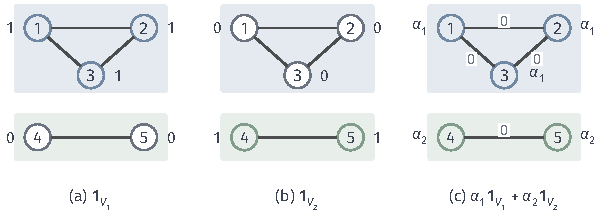
\includegraphics{figures/03-graphs/05-matrices-and-spectra/tikz/incidence-component-constants/figure.pdf}
  \caption{含$c=2$个连通分量$V_1=\{1,2,3\}$（蓝底）与$V_2=\{4,5\}$（绿底）的五点图上$\ker\bm{B}^\top$的基与通解。(a) 第一分量指示向量$\bm{1}_{V_1}=(1,1,1,0,0)^\top$。(b) 第二分量指示向量$\bm{1}_{V_2}=(0,0,0,1,1)^\top$。(c) 一般零空间向量$\bm{f}=\alpha_1\bm{1}_{V_1}+\alpha_2\bm{1}_{V_2}$在两个分量上分别取独立常数$\alpha_1,\alpha_2$，每条边的两端同属一个分量，沿边差分全为$0$。}
  \label{fig:incidence-component-constants}
\end{BookInlineFigure}

有了$\dim\ker\bm{B}^\top=c$，连续使用两次线性代数的秩零度定理（rank-nullity theorem），即可直接导出关联矩阵的秩以及割空间、环空间的维数公式。

\begin{theorem}[环空间与割空间的维数]
\label{thm:incidence-cycle-cut-dimensions}
设有限图$\mathcal{G}=(V,E)$有$n$个顶点、$m$条边和$c$个连通分量，关联矩阵为$\bm{B}\in\mathbb{R}^{n\times m}$。则关联矩阵的秩为
\begin{equation}
\operatorname{rank}\bm{B}=\operatorname{rank}\bm{B}^\top=n-c,
\label{eq:incidence-rank-components}
\end{equation}
且割空间$\mathcal{D}(\mathcal{G})=\operatorname{im}\bm{B}^\top$与环空间$\mathcal{C}(\mathcal{G})=\ker\bm{B}$的维数分别为
\begin{equation}
\dim\mathcal{D}(\mathcal{G})=n-c,\qquad
\dim\mathcal{C}(\mathcal{G})=m-n+c.
\label{eq:incidence-cycle-cut-dimensions}
\end{equation}
\end{theorem}

\begin{proof}
首先考察沿边差分算子$\bm{B}^\top\colon\mathbb{R}^V\to\mathbb{R}^E$。它的定义域是$n$维顶点空间$\mathbb{R}^V$，零空间$\ker\bm{B}^\top$由$c$个连通分量的指示向量$\{\bm{1}_{V_1},\ldots,\bm{1}_{V_c}\}$张成且线性无关，故$\dim\ker\bm{B}^\top=c$。对线性映射$\bm{B}^\top$应用秩零度定理，其像空间$\mathcal{D}(\mathcal{G})=\operatorname{im}\bm{B}^\top$的维数为
\[
\dim\mathcal{D}(\mathcal{G})=\operatorname{rank}\bm{B}^\top=\dim\mathbb{R}^V-\dim\ker\bm{B}^\top=n-c.
\]
由于矩阵与其转置的秩相等，有$\operatorname{rank}\bm{B}=\operatorname{rank}\bm{B}^\top=n-c$，式~\eqref{eq:incidence-rank-components}得证。

再考察净流出汇总算子$\bm{B}\colon\mathbb{R}^E\to\mathbb{R}^V$。它的定义域是$m$维边空间$\mathbb{R}^E$，秩为$\operatorname{rank}\bm{B}=n-c$。对$\bm{B}$应用秩零度定理，其零空间$\mathcal{C}(\mathcal{G})=\ker\bm{B}$的维数为
\[
\dim\mathcal{C}(\mathcal{G})=\dim\ker\bm{B}=\dim\mathbb{R}^E-\operatorname{rank}\bm{B}=m-(n-c)=m-n+c.
\]
式~\eqref{eq:incidence-cycle-cut-dimensions}得证。
\end{proof}

验证两个具体情形：在图~\ref{fig:incidence-running-example}的四点五边图上，$n=4,m=5,c=1$，由定理~\ref{thm:incidence-cycle-cut-dimensions}立得割空间维数为$4-1=3$，环空间维数为$5-4+1=2$，两者之和$3+2=5=m$，与正交直和分解式~\eqref{eq:incidence-edge-space-decomposition}完全吻合。

又若图$\mathcal{G}$是一片不含任何环的森林（forest），则边数恰为$m=n-c$，此时环空间维数$\dim\mathcal{C}(\mathcal{G})=(n-c)-n+c=0$，即森林上不存在任何非零环流。直观上，无环图中任何非零流量一旦沿某条边流出，最终必然到达度为$1$的叶子顶点而无法绕回，从而在叶子处破坏流量守恒。下一小节将利用生成森林把这一观察转化为显式基的构造与证明。

\subsection{基本环基}
\label{sec:incidence-fundamental-bases}

定理~\ref{thm:incidence-cycle-cut-dimensions}给出了环空间维数$m-n+c$和割空间维数$n-c$，但还没有具体指明怎样找出一组基向量。注意到在一张有$n$个顶点、$c$个连通分量的图$\mathcal{G}=(V,E)$中，任取一棵生成森林$F\subseteq E$（当图连通、$c=1$时就是一棵生成树$T$），森林$F$中包含的\emph{树边}（tree edges）条数恰好是$n-c$，等于割空间的维数；而留在森林之外的\emph{非树边}（non-tree edges，也称弦，$E\setminus F$）条数恰好是$m-(n-c)=m-n+c$，等于环空间的维数。

这并非巧合：用每条非树边与树路径闭合，可以逐一构造出$m-n+c$个线性无关的基本环向量；下一小节再逐一删去每条树边将生成树切成两半，构造出$n-c$个线性无关的基本割向量。

下面说明如何由生成森林$F$和每一条非树边$e\in E\setminus F$构造基本环向量。取定一条非树边$e\colon u\to v\in E\setminus F$，由于$e$的两个端点$u$和$v$属于同一个连通分量，在生成森林$F$内部已经存在唯一一条连接$v$到$u$的树路径$P_e\subseteq F$；将非树边$e$添入$F$中，边集$P_e\cup\{e\}$就构成唯一一个简单环，记为$C_e$。规定沿环$C_e$的绕行方向与非树边$e$本身的参考方向$u\to v$一致（即先沿$e$从$u$走到$v$，再沿树路径$P_e$从$v$走回$u$），据此定义一个边流量向量$\bm{c}^{(e)}\in\mathbb{R}^E$：
\[
\bigl(\bm{c}^{(e)}\bigr)_{e'}=
\begin{cases}
+1,& e'=e\text{（即该非树边本身）},\\[2pt]
+1,& e'\in P_e\text{ 且 }e'\text{ 的参考方向与 }C_e\text{ 的绕行方向一致},\\[2pt]
-1,& e'\in P_e\text{ 且 }e'\text{ 的参考方向与 }C_e\text{ 的绕行方向相反},\\[2pt]
0,& e'\notin C_e\text{（包括其余所有非树边及不在 }P_e\text{ 上的树边）}.
\end{cases}
\]
向量$\bm{c}^{(e)}$称为对应于非树边$e$的\term{基本环}向量（fundamental cycle vector）。

我们在图~\ref{fig:incidence-running-example}的四点五边图上演示这一构造过程。如图~\ref{fig:incidence-fundamental-cycles}(a)所示，选取路径生成树$T=\{12,23,34\}$（共$n-1=3$条树边），留下的两条非树边为$E\setminus T=\{41,13\}$（共$m-n+1=2$条非树边）。

先添入非树边$41$（参考方向$4\to1$）：如图~\ref{fig:incidence-fundamental-cycles}(b)所示，沿非树边$41$从$4$走到$1$，再沿树路径$1\to2\to3\to4$返回$4$。沿途经过的三条树边$12,23,34$均与各自的参考方向同向（各取$+1$），另一条非树边$13$不在环上（取$0$），按边序$(12,23,34,41,13)$得到第一个基本环向量
\[
\bm{c}_1=\bm{c}^{(41)}=(1,1,1,\;1,0)^\top.
\]
再添入非树边$13$（参考方向$1\to3$）：如图~\ref{fig:incidence-fundamental-cycles}(c)所示，沿非树边$13$从$1$走到$3$，再沿树路径$3\to2\to1$返回$1$。返回途中经过的树边$23$和$12$均与各自的参考方向（$2\to3$和$1\to2$）相反，分量均取$-1$；树边$34$和另一条非树边$41$不在环上，均取$0$，得到第二个基本环向量
\[
\bm{c}_2=\bm{c}^{(13)}=(-1,-1,0,\;0,1)^\top.
\]

\begin{BookInlineFigure}
  \centering
  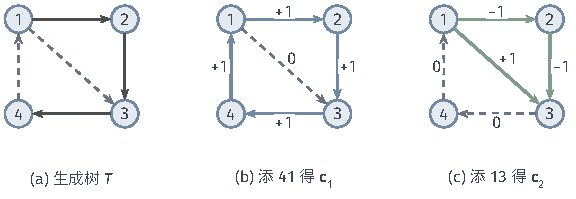
\includegraphics{figures/03-graphs/05-matrices-and-spectra/tikz/incidence-fundamental-cycles/figure.pdf}
  \caption{在四点五边图上由路径生成树$T=\{12,23,34\}$构造基本环基。(a) 实线为三条树边$12,23,34$，虚线为两条非树边$41,13$。(b) 添入非树边$41$并沿树路径$1\to2\to3\to4$闭合，得到基本环向量$\bm{c}_1=(1,1,1,1,0)^\top$。(c) 添入非树边$13$并沿树路径$3\to2\to1$闭合（逆参考方向经过$23$与$12$），得到基本环向量$\bm{c}_2=(-1,-1,0,0,1)^\top$。}
  \label{fig:incidence-fundamental-cycles}
\end{BookInlineFigure}

观察$\bm{c}_1$和$\bm{c}_2$在最后两个坐标——即两条非树边$(41,13)$——上的取值：$\bm{c}_1$在$(41,13)$处为$(1,0)^\top$，$\bm{c}_2$在$(41,13)$处为$(0,1)^\top$，拼在一起恰好是$2\times 2$单位矩阵$\bigl(\begin{smallmatrix}1&0\\0&1\end{smallmatrix}\bigr)$。每条非树边只出现在它自己生成的那个基本环中，而在其他所有基本环中坐标全为$0$。正是这一“非树边坐标呈单位阵”的结构，使基本环向量的线性无关性与坐标展开变得可以直接验证。

\begin{theorem}[基本环基]
\label{thm:incidence-fundamental-cycle-basis}
设有限图$\mathcal{G}=(V,E)$有$n$个顶点、$m$条边和$c$个连通分量，$F\subseteq E$为其一棵生成森林。则由$m-n+c$条非树边$e\in E\setminus F$构造的基本环向量集合
\[
\bigl\{\bm{c}^{(e)}:e\in E\setminus F\bigr\}
\]
构成环空间$\mathcal{C}(\mathcal{G})=\ker\bm{B}$的一组基。特别地，任意环流$\bm{q}\in\mathcal{C}(\mathcal{G})$均可按其在非树边上的分量唯一展开为
\begin{equation}
\bm{q}=\sum_{e\in E\setminus F}q_e\,\bm{c}^{(e)}.
\label{eq:incidence-fundamental-cycle-expansion}
\end{equation}
\end{theorem}

\begin{proof}
我们分三步证明：（1）每个$\bm{c}^{(e)}$属于$\mathcal{C}(\mathcal{G})$；（2）这$m-n+c$个向量线性无关；（3）任意环流$\bm{q}\in\mathcal{C}(\mathcal{G})$均满足展开式~\eqref{eq:incidence-fundamental-cycle-expansion}。

\textbf{第一步（属于环空间）}：对每条非树边$e\in E\setminus F$，$C_e$是一个简单闭合回路。不在$C_e$上的顶点关联的边流量全为$0$，净流出量为$0$；在$C_e$上的每个顶点恰好作为$C_e$中一条边的流入端和另一条边的流出端，按绕行方向一进一出各$1$个单位，根据关联矩阵作用公式~\eqref{eq:incidence-net-outflow}，其净流出量也为$1-1=0$。因此$\bm{B}\bm{c}^{(e)}=\bm{0}$，即$\bm{c}^{(e)}\in\mathcal{C}(\mathcal{G})$。

\textbf{第二步（线性无关）}：设有一组实系数$\{\alpha_e:e\in E\setminus F\}$使得
\[
\sum_{e'\in E\setminus F}\alpha_{e'}\,\bm{c}^{(e')}=\bm{0}.
\]
任取一条非树边$e\in E\setminus F$，读取上式两端在第$e$条边上的坐标分量。由基本环向量的构造规则，$\bm{c}^{(e)}$在边$e$上的分量为$1$，而其余所有基本环向量$\bm{c}^{(e')}$（$e'\neq e$）在非树边$e$上的分量全为$0$。因此上式左端在第$e$条边上的分量就是$\alpha_e\cdot 1+0=\alpha_e$，右端为$0$，故$\alpha_e=0$。对每条非树边$e\in E\setminus F$均如此，说明$\{\bm{c}^{(e)}:e\in E\setminus F\}$线性无关。

\textbf{第三步（张成性与唯一展开式）}：由定理~\ref{thm:incidence-cycle-cut-dimensions}，环空间的维数为$\dim\mathcal{C}(\mathcal{G})=m-n+c$，因此$\mathcal{C}(\mathcal{G})$中$m-n+c$个线性无关的向量已经构成一组基。为了直接导出展开式~\eqref{eq:incidence-fundamental-cycle-expansion}，任取环流$\bm{q}\in\ker\bm{B}$，直接用$\bm{q}$在各条非树边上的分量$q_e$作系数，构造余量向量
\[
\bm{r}=\bm{q}-\sum_{e\in E\setminus F}q_e\,\bm{c}^{(e)}.
\]
一方面，$\bm{r}$是环流的线性组合，故仍满足守恒条件$\bm{B}\bm{r}=\bm{0}$；另一方面，在每一条非树边$e\in E\setminus F$上，$r_e=q_e-q_e\cdot 1=0$。这意味着守恒流$\bm{r}$在所有非树边上全为零，只可能在生成森林$F$的树边上非零。

若$\bm{r}\neq\bm{0}$，设$F'\subseteq F$为$r_{e'}\neq 0$的树边子集。因为$F'$是森林的非空子图（无环），$F'$中必然存在一个只与$F'$中唯一一条边$e_1\in F'$相连的叶子顶点$v$。但在顶点$v$处，$\bm{r}$在关联于$v$的其余所有边上分量皆为$0$，故净流出量为$(\bm{B}\bm{r})_v=\pm r_{e_1}$；由守恒条件$(\bm{B}\bm{r})_v=0$立得$r_{e_1}=0$，与$e_1\in F'$矛盾。（等价地，从生成森林$F$的叶子顶点开始逐次剥去叶子与所连树边，每一步叶子处的守恒方程都迫使该树边流量为零，直至整片森林清空。）因此必有$\bm{r}=\bm{0}$，式~\eqref{eq:incidence-fundamental-cycle-expansion}得证。
\end{proof}

\subsection{基本割基}
\label{sec:incidence-fundamental-cut-bases}

与非树边生成基本环对偶，生成森林$F$中的每一条树边$e\in F$都可以用来构造一个基本割向量。取定一条树边$e\colon u\to v\in F$，设它属于连通分量$V_k$的生成树$T_k$。因为树是连通无环图，从$T_k$中删去树边$e$后，$T_k$恰好分裂成两棵互不连通的子树；取包含边$e$尾端$u$的那棵子树的顶点集为$S_e$（头端$v$落在另一侧$V\setminus S_e$中），以子集$S_e$的指示向量$\bm{1}_{S_e}\in\mathbb{R}^V$作用沿边差分算子$\bm{B}^\top$，定义
\[
\bm{d}^{(e)}=\bm{B}^\top\bm{1}_{S_e}\in\mathbb{R}^E.
\]
考察$\bm{d}^{(e)}$在各条边上的分量：在被删的树边$e\colon u\to v$本身上，尾端$u\in S_e$（读数$1$）、头端$v\notin S_e$（读数$0$），故$\bigl(\bm{d}^{(e)}\bigr)_e=1-0=+1$；在生成森林的其余所有树边$e'\in F\setminus\{e\}$上，删去$e$并没有切断$e'$，因此$e'$的两个端点必定同在$S_e$内或同在$S_e$外，两端读数相等，故$\bigl(\bm{d}^{(e)}\bigr)_{e'}=0$；在原图的非树边$e''\in E\setminus F$上，若$e''$跨越$S_e$与$V\setminus S_e$，则按参考方向从$S_e$穿出取$+1$、穿入取$-1$，不跨割则取$0$。向量$\bm{d}^{(e)}$称为对应于树边$e\in F$的\term{基本割}向量（fundamental cut vector）。

仍在四点五边图的路径生成树$T=\{12,23,34\}$上逐一构造全部$n-1=3$个基本割向量（边序仍为$12,23,34,41,13$），如图~\ref{fig:incidence-tree-cycle-cut}所示。

删去树边$12$（$1\to2$）时（图~\ref{fig:incidence-tree-cycle-cut}(a)），树$T$分裂为尾端侧$S_1=\{1\}$与头端侧$\bar{S}_1=\{2,3,4\}$，树边$12$从$S_1$指向$\bar{S}_1$（取$+1$），其余两条树边$23,34$两端都在$\bar{S}_1$内（取$0$），非树边$41$从$4$指向$1$（取$-1$），非树边$13$从$1$指向$3$（取$+1$），得到第一个基本割向量$\bm{d}_1=\bm{d}^{(12)}$。

删去树边$23$（$2\to3$）时（图~\ref{fig:incidence-tree-cycle-cut}(b)），树$T$分裂为$S_2=\{1,2\}$与$\bar{S}_2=\{3,4\}$，树边$23$取$+1$、树边$12,34$取$0$，非树边$41$取$-1$、$13$取$+1$，得到第二个基本割向量$\bm{d}_2=\bm{d}^{(23)}$。

删去树边$34$（$3\to4$）时（图~\ref{fig:incidence-tree-cycle-cut}(c)），树$T$分裂为$S_3=\{1,2,3\}$与$\bar{S}_3=\{4\}$，树边$34$取$+1$、树边$12,23$取$0$，非树边$41$从$4$进入$1$（取$-1$），非树边$13$两端都在$S_3$内（取$0$），得到第三个基本割向量$\bm{d}_3=\bm{d}^{(34)}$。三个基本割向量依次为
\[
\bm{d}_1=(1,0,0,\;-1,1)^\top,\quad
\bm{d}_2=(0,1,0,\;-1,1)^\top,\quad
\bm{d}_3=(0,0,1,\;-1,0)^\top.
\]

\begin{BookInlineFigure}
  \centering
  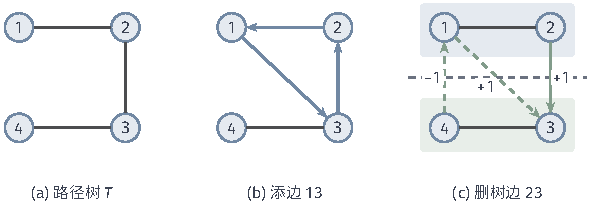
\includegraphics{figures/03-graphs/05-matrices-and-spectra/tikz/incidence-tree-cycle-cut/figure.pdf}
  \caption{在四点五边图上由路径生成树$T=\{12,23,34\}$构造三个基本割基向量。每个面板删去一条树边，蓝底标出含该树边尾端的子树顶点集$S_k$，绿底标出另一侧$\bar{S}_k$；绿实线（$+1$）和红实线（$-1$）为跨割边，灰虚线（$0$）为同侧边。(a) 删树边$12$，$S_1=\{1\}$，得$\bm{d}_1=(1,0,0,-1,1)^\top$。(b) 删树边$23$，$S_2=\{1,2\}$，得$\bm{d}_2=(0,1,0,-1,1)^\top$。(c) 删树边$34$，$S_3=\{1,2,3\}$，得$\bm{d}_3=(0,0,1,-1,0)^\top$。}
  \label{fig:incidence-tree-cycle-cut}
\end{BookInlineFigure}

观察$\bm{d}_1,\bm{d}_2,\bm{d}_3$在前三个坐标——即三条树边$(12,23,34)$——上的取值：它们依次为$(1,0,0)^\top,(0,1,0)^\top,(0,0,1)^\top$，拼在一起恰好是$3\times 3$单位矩阵。每条树边只出现在删去它自己时生成的那个基本割中，而在其余基本割中分量全为$0$。据此可立即证明基本割基定理。

\begin{theorem}[基本割基]
\label{thm:incidence-fundamental-cut-basis}
设有限图$\mathcal{G}=(V,E)$有$n$个顶点、$m$条边和$c$个连通分量，$F\subseteq E$为其一棵生成森林。则由$n-c$条树边$e\in F$构造的基本割向量集合
\[
\bigl\{\bm{d}^{(e)}:e\in F\bigr\}
\]
构成割空间$\mathcal{D}(\mathcal{G})=\operatorname{im}\bm{B}^\top$的一组基。特别地，任意割差分向量$\bm{d}\in\mathcal{D}(\mathcal{G})$均可按其在树边上的分量唯一展开为
\begin{equation}
\bm{d}=\sum_{e\in F}d_e\,\bm{d}^{(e)}.
\label{eq:incidence-fundamental-cut-expansion}
\end{equation}
\end{theorem}

\begin{proof}
首先，每个$\bm{d}^{(e)}=\bm{B}^\top\bm{1}_{S_e}$由顶点函数$\bm{1}_{S_e}$经$\bm{B}^\top$作用生成，故属于$\mathcal{D}(\mathcal{G})=\operatorname{im}\bm{B}^\top$。

其次证明线性无关。设有一组实系数$\{\beta_e:e\in F\}$使得
\[
\sum_{e'\in F}\beta_{e'}\,\bm{d}^{(e')}=\bm{0}.
\]
任取一条树边$e\in F$，读取上式两端在第$e$条边上的坐标分量。由基本割向量的构造规则，$\bm{d}^{(e)}$在树边$e$上的分量为$1$，而其余所有基本割向量$\bm{d}^{(e')}$（$e'\in F\setminus\{e\}$）在树边$e$上的分量全为$0$。因此左端在树边$e$处的分量就是$\beta_e\cdot 1+0=\beta_e$，右端为$0$，故$\beta_e=0$。这证明了$n-c$个基本割向量线性无关。

最后，由定理~\ref{thm:incidence-cycle-cut-dimensions}知割空间的维数为$\dim\mathcal{D}(\mathcal{G})=n-c$。在$n-c$维空间中，$n-c$个线性无关的向量$\{\bm{d}^{(e)}:e\in F\}$必然构成一组基。因此，任意$\bm{d}\in\mathcal{D}(\mathcal{G})$都可唯一展开为$\bm{d}=\sum_{e'\in F}\beta_{e'}\bm{d}^{(e')}$；读取两端在每条树边$e\in F$上的坐标分量，立得$d_e=\beta_e$，即展开式~\eqref{eq:incidence-fundamental-cut-expansion}成立。
\end{proof}

\paragraph{正交性的验证}

我们可以用四点五边图上求出的基本环基$\{\bm{c}_1,\bm{c}_2\}$与基本割基$\{\bm{d}_1,\bm{d}_2,\bm{d}_3\}$直接核对环空间与割空间的正交性。例如，取基本割向量$\bm{d}_2=(0,1,0,-1,1)^\top$，将其分别与$\bm{c}_1$和$\bm{c}_2$作内积：
\[
\begin{aligned}
\bm{c}_1^\top\bm{d}_2&=1\cdot0+1\cdot1+1\cdot0+1\cdot(-1)+0\cdot1=1-1=0,\\
\bm{c}_2^\top\bm{d}_2&=(-1)\cdot0+(-1)\cdot1+0\cdot0+0\cdot(-1)+1\cdot1=-1+1=0.
\end{aligned}
\]
从图上看，任何一个基本环一旦跨过基本割从$S_e$进入$\bar{S}_e$（贡献一次树边或非树边同向乘积），为了回到起点就必须再次跨过该割从$\bar{S}_e$返回$S_e$（贡献一次反向乘积），两次跨割的乘积符号相反、恰好成对抵消。

最后指出，换选另一棵生成树（或生成森林）会得到另一套基本环基和基本割基，基向量的具体坐标随之改变；但它们所张成的环空间$\mathcal{C}(\mathcal{G})=\ker\bm{B}$和割空间$\mathcal{D}(\mathcal{G})=\operatorname{im}\bm{B}^\top$本身只由原图的关联矩阵$\bm{B}$唯一确定，不随生成树的选择而改变。
